\section{Resultados}
\label{sec:resultados}

\subsection{Distribuci\'on de los factores}

Sobre las 210 presas del cat\'alogo, el PGA vari\'o entre 0.0085$g$ y 0.735$g$ (mediana 0.104$g$), la lluvia de dise\~no a 100 a\~nos entre 40.4 mm y 211.2 mm/d\'ia (mediana 60.2 mm/d\'ia), y la poblaci\'on en 30 km entre 456 y 28.4 millones de habitantes (mediana 198{,}658), esta \'ultima con una asimetr\'ia much\'isimo mayor que los otros dos factores --consistente con que la poblaci\'on se concentra en un n\'umero peque\~no de zonas metropolitanas grandes--.

\subsection{Independencia entre factores}

La correlaci\'on de Pearson entre los percentiles de los tres factores fue baja: 0.086 entre el s\'ismico y el hidrol\'ogico, 0.290 entre el s\'ismico y el poblacional, y $-0.301$ entre el hidrol\'ogico y el poblacional. Esta independencia relativa es deseable: confirma que los tres factores capturan dimensiones de riesgo distintas y que el \'indice compuesto (Ecuaci\'on \ref{eq:indice}) no est\'a dominado impl\'icitamente por una sola de ellas.

\subsection{Ranking de prioridad}

La Tabla \ref{tab:top10} reporta las diez presas con mayor \'indice de prioridad. El resultado no reproduce un ranking dominado por un solo criterio geogr\'afico: combina presas de la zona de subducci\'on de la costa del Pac\'ifico y el sureste --Manuel Moreno Torres (Chiapas), La Cangrejera (Veracruz), Jos\'e Mar\'ia Morelos y Pav\'on (Michoac\'an)--, cuyo peso proviene principalmente del peligro s\'ismico e hidrol\'ogico, con presas de sismicidad moderada pero muy alta densidad poblacional cercana --El Carrizo y Abelardo L. Rodr\'iguez, ambas en la zona metropolitana de Tijuana, Baja California; Manuel \'Avila Camacho, cerca de la zona metropolitana de Puebla--.

\begin{table}[htbp]
\centering
\caption{Top 10 presas por \'indice de prioridad de revisi\'on}
\label{tab:top10}
\begin{tabular}{@{}llr@{}}
\toprule
Clave & Estado & \'Indice \\
\midrule
CHICP & Chiapas & 88.3 \\
LCAVC & Veracruz & 87.6 \\
CRRBN & Baja California & 82.1 \\
SOLPB & Puebla & 82.0 \\
BDDPB & Puebla & 81.8 \\
ALRBN & Baja California & 81.6 \\
VILMC & Michoac\'an & 81.5 \\
SNLSI & Sinaloa & 80.1 \\
ELZBN & Baja California & 77.9 \\
COIMC & Michoac\'an & 77.6 \\
\bottomrule
\end{tabular}
\end{table}

La Figura \ref{fig:mapa} muestra el \'indice de prioridad geogr\'aficamente. Las presas de menor prioridad se concentran en el altiplano central --zona de baja sismicidad y lluvia moderada--, mientras que las de mayor prioridad se distribuyen en la periferia del pa\'is: la costa del Pac\'ifico y el sureste por peligro combinado, y los n\'ucleos urbanos grandes (frontera norte, Puebla) por exposici\'on poblacional.

\begin{figure}[htbp]
\centering
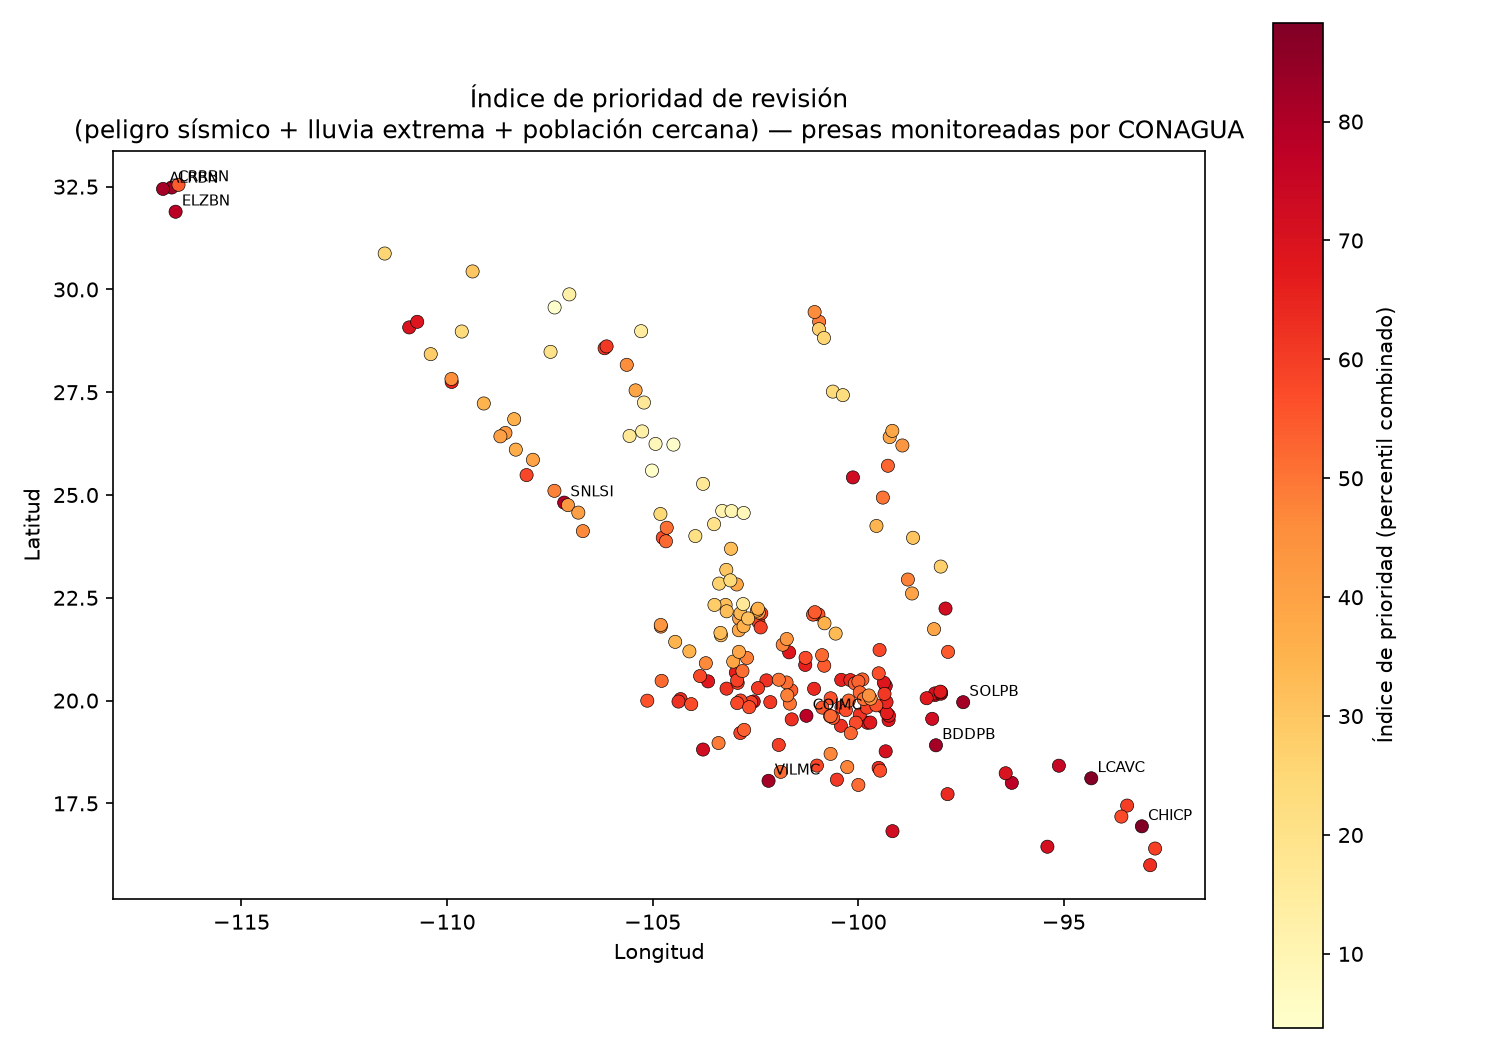
\includegraphics[width=\columnwidth]{figures/mapa_prioridad_presas.png}
\caption{\'Indice de prioridad de revisi\'on por presa (peligro s\'ismico + lluvia extrema + poblaci\'on cercana), 210 presas monitoreadas por CONAGUA.}
\label{fig:mapa}
\end{figure}
